\documentclass[a4paper]{article}
\usepackage{siunitx}
\usepackage{amsmath}
\usepackage{graphicx}
\usepackage{subfigure}
\usepackage{hyperref}
\usepackage{indentfirst}


\usepackage{geometry}
\geometry{a4paper,scale=0.8} % 调整页边距
% 插入代码
\usepackage{listings}
\usepackage{xcolor}
\lstset{
 columns=fixed,
 % basicstyle=\tiny,
 numbers=right,                                        % 在左侧显示行号
 numberstyle=\tiny\color{gray},                       % 设定行号格式
 frame=single,                                          % 不显示背景边框
 backgroundcolor=\color[RGB]{245,245,244},            % 设定背景颜色
 keywordstyle=\color[RGB]{40,40,255},                 % 设定关键字颜色
 numberstyle=\footnotesize\color{darkgray},           
 commentstyle=\it\color[RGB]{0,96,96},                % 设置代码注释的格式
 stringstyle=\rmfamily\slshape\color[RGB]{128,0,0},   % 设置字符串格式
 showstringspaces=false,                              % 不显示字符串中的空格
 language=matlab,                                        % 设置语言
 breaklines=true                                      % 换行
}



\author{Shi Yongxiang\footnote{Shi Yongxiang, the KAUST Visiting Sutdent in CSIM, email: yongxiang.shi@kaust.edu.sa}}
\title{WEB\_LABS reading report}
\begin{document}
	
	\maketitle

\section{FD, a2d\_mod\_abc28\_snapshot.m}
	\textbf{a2d\_mod\_abc28\_snapshot.m}
	this is a program to solve a acoustic wave equation with accuracy of 2-8 while using the absorbing boundary conditions. To achieve it, we need functions to deal with:

	\begin{itemize}
		\item[1] \textbf{Boundary condition}. When we use FD, to simulate the waveform equation, we need to deal the boundary for the finite computation area.
		\item[2] \textbf{Source} How to generate the source, and how to put a source at a location and activate the waveform.
		\item[3] \textbf{Propragate} We will use 2D 8-Order FD to calculate it
	\end{itemize}

	\subsection{Boundary Condition - ABC}
		 To deal the reflection on four boundaries, we set absrobing area at the edge of target. Codes was shown in \autoref{ABCcode}. 
		 First, we need extend the vel with zeros at the edge area. The we need to get a special variable \textbf{damp} to store the ABC settings. 
		 When we get the variable of \textbf{damp}, we can plot it in \autoref{ABCfigure}. 
		 In the extended areas, \textbf{damp} was set as

		 $$damp_{1d}=C\times(\frac{d_{i2b}}{D_{abc}})^2,C: C_0\times v_{min}/D_{abc}$$,

		 where $C_0$ is a big constant; $d_{i2b}/D_{abc}$ is the normalized distance to boundary.remeber, at this time, values in damp do not have physical meaning.

		\begin{lstlisting}[caption=set ABC to the velocity variable (2 is same), label=ABCcode]

% divide the whole area to 9 zones, and 5th is the target zone
%  1   |   2   |   3
%  ------------------
%  4   |   5   |   6
%  ------------------
%  7   |   8   |   9
[nzbc,nxbc]=vel_expended
% fulltill zone 1, 4, 7 and 3, 6, 9
for iz=1:nzbc
    damp(iz,1:nbc)=damp1d(nbc:-1:1);
    damp(iz,nx+nbc+1:nx+2*nbc)=damp1d(:);
end
% full fill zone 2 and 8
for ix=nbc+1:nbc+nx
    damp(1:nbc,ix)=damp1d(nbc:-1:1);
    damp(nbc+nz+1:nz+2*nbc,ix)=damp1d(:);
end
	    \end{lstlisting}

		\begin{figure}
			\centering
			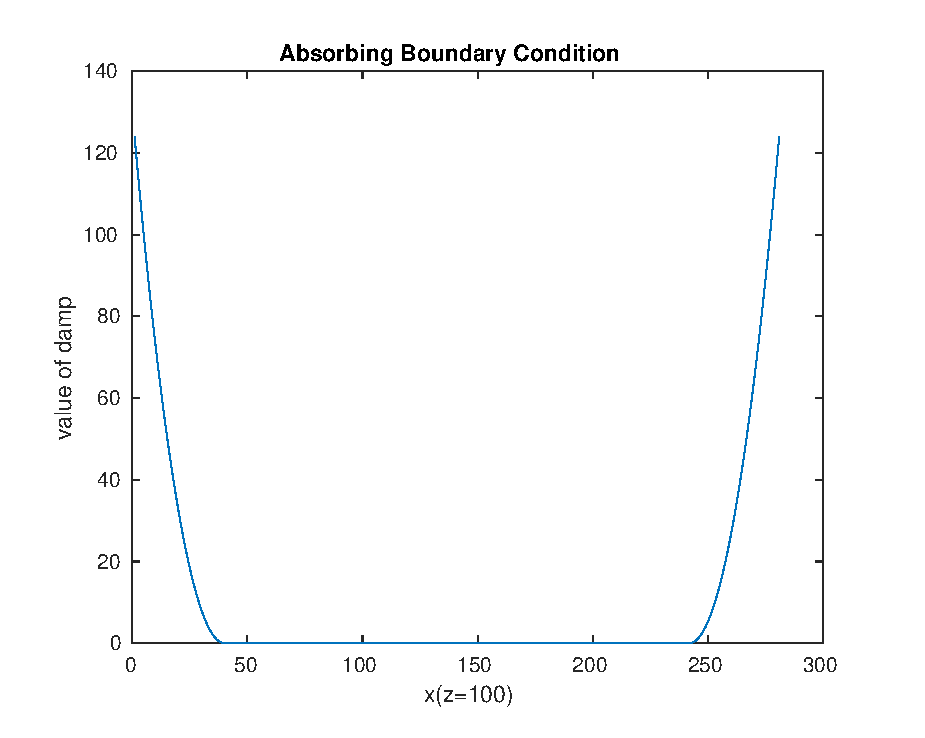
\includegraphics[width=0.5\linewidth]{fig/ABC.eps}
			\caption{ABC example}
			\label{ABCfigure}
		\end{figure}

	\subsection{Source - ricker wavelet}
		the expression of ricker wavelet is \autoref{ricker}:
		\begin{equation}
			\begin{aligned}
				IN: & f, \Delta t, nt\\
				OUT:& r = \sum_{-n}^{n}(1-2\alpha_i^2 )e^{- \alpha_i^2 }, n = \frac{1.1}{f\Delta t}, \alpha_i = if\Delta t * \pi
			\end{aligned}
			\label{ricker}
			\centering
		\end{equation}
		After we generate this ricker wavelet, we can enlength it by appending zeros. In this way, we can get a verctor of source, which's header is a ricker wavelet with f freq and $\Delta t$.
	
	\subsection{Propagate - FD}

		First, we need figure out how to get a approximate expression of the 2-order partial derivative. Using Tylor series, we can get a result as:
			$$f''(x)=\sum_{-n}^{n}c_{i}f(x+i\Delta x) + o(\Delta x ^{2n+1})$$
		and we call it as the n-order approximation of the fuction. to be simple, we let $c_i=c_{-i}$, then we need solve \autoref{n-order}:

		\begin{equation}
			\begin{bmatrix}
				\frac{1^2}{2!} & \frac{2^2}{2!} & \ldots & \frac{n^2}{2!}\\
				\frac{1^4}{4!} & \frac{2^4}{4!} & \ldots & \frac{n^4}{4!}\\
				\vdots & \vdots & \ddots & \vdots\\
				\frac{1^{2n}}{2n!} & \frac{2^{2n}}{2n!} & \ldots & \frac{n^{2n}}{2n}
			\end{bmatrix}
			\begin{bmatrix}
				 c_1\\c_2\\\vdots\\c_n
			\end{bmatrix}
			=
			\begin{bmatrix}
				 1\\0\\\vdots\\0
			\end{bmatrix}
			\label{n-order}
		\end{equation}
		 and we have $c_0=-2 \sum_{i=1}^{n}c_i$.

		When getting the expression of \textbf{$c_i$}, express the waveform equation as:\autoref{FD-n}, and \autoref{FD-ABC} with ABC.
		\begin{align}
			&(\frac{v\Delta t}{\Delta x})^2\sum_{i=1}^n c_i[p_t(x+i\Delta x,z)+p_t(x-i\Delta x, z)] \notag\\
			+&(\frac{v\Delta t}{\Delta z})^2\sum_{i=1}^n c_i[p_t(x, z+i\Delta z)+p_t(x, -i\Delta z)] \notag\\
			+&[(\frac{v\Delta t}{\Delta x})^2c_0+(\frac{v\Delta t}{\Delta z})^2c_0+2]p_t(x,z)\notag\\
			+&2p_t(x,z)-p_{t-1}(x,z)=p_{t+1}(x,z)
			\label{FD-n}
		\end{align}

		\begin{align}
			&(\frac{v\Delta t}{\Delta x})^2\sum_{i=1}^n c_i[p_t(x+i\Delta x,z)+p_t(x-i\Delta x, z)] \notag\\
			+&(\frac{v\Delta t}{\Delta z})^2\sum_{i=1}^n c_i[p_t(x, z+i\Delta z)+p_t(x, -i\Delta z)] \notag\\
			+&[(\frac{v\Delta t}{\Delta x})^2c_0+(\frac{v\Delta t}{\Delta z})^2c_0+2]p_t(x,z)\notag\\
			+&(2-\kappa)p_t(x,z)-(1-\kappa)p_{t-1}(x,z)=p_{t+1}(x,z) \notag\\
			,&where\ \kappa=(\frac{d_{i2b}}{D_{abc}})^2\times 3.0 \times  16 v_{min}\times \Delta t 
			\label{FD-ABC}			
		\end{align}

		And the program language is as \autoref{FDCode} shows\footnote{why $p(isz,isx) = p(isz,isx) + beta_dt(isz,isx) * s(it)$}
		\begin{lstlisting}[caption=set ABC to the velocity variable (2 is same), label=FDCode,basicstyle=\tiny, numberstyle=\tiny]
% 
alpha=(v*dt/dx).^2; kappa=damp*dt;
for it=1:nt
	p=(2+2*c0*alpha-kappa).*p1-(1-kappa).*p0+alpha.*...
	(c1*(circshift(p1,[0,1,0])+circshift(p1,[0,-1,0])+circshift(p1,[1,0,0])+circshift(p1,[-1,0,0]))...
	+c2*(circshift(p1,[0,2,0])+circshift(p1,[0,-2,0])+circshift(p1,[2,0,0])+circshift(p1,[-2,0,0]))...
	+c3*(circshift(p1,[0,3,0])+circshift(p1,[0,-3,0])+circshift(p1,[3,0,0])+circshift(p1,[-3,0,0]))...
	+c4*(circshift(p1,[0,4,0])+circshift(p1,[0,-4,0])+circshift(p1,[4,0,0])+circshift(p1,[-4,0,0]))); 
	% here dx=dz, and c0=c1, c1=c2...
	% if free boundary at the bottom
	if isFS
		p(nbc+1,:)=0.0;
		p(nbc:-1:nbc-3,:) = - p(nbc+2:nbc+5,:);
	end
	% add source
	p(isz,isx) = p(isz,isx) + beta_dt(isz,isx) * s(it);
	p1,p0=p,p1;
end
    	\end{lstlisting}


\section{RTM, a2d\_rtm\_abc28\_snapshot.m}	
	this is a section to realize the RTM(reverse time migration) method.According the introduction in \cite[Schuster 2015]{SI}. There are some aspects:

	\begin{itemize}
		\item[1] \textbf{how to calculate the backpropagated wavefield?} To get the image of RTM , we need the corelation of the wavefield from source and the backpropagated wavefield from geophones,but how to get the backpropagated wavefield? Does the Green function's reciprocity work?
		\item[2] \textbf{how to get the approximated velocity?} The wavefield from source is required to be a down-going propagation, so what features of veolicity are need to get the down-going wavefield?
	\end{itemize}

	\subsection{get the simuation Data and Smooth velocity}

	We could use the FD method in section 1 to get the simuation seismic data in geophones, as \autoref{rtm_simD} shows. Smoothed velocity means that the interface becomes not so sharp?

	\begin{figure}[ht]
		\centering
		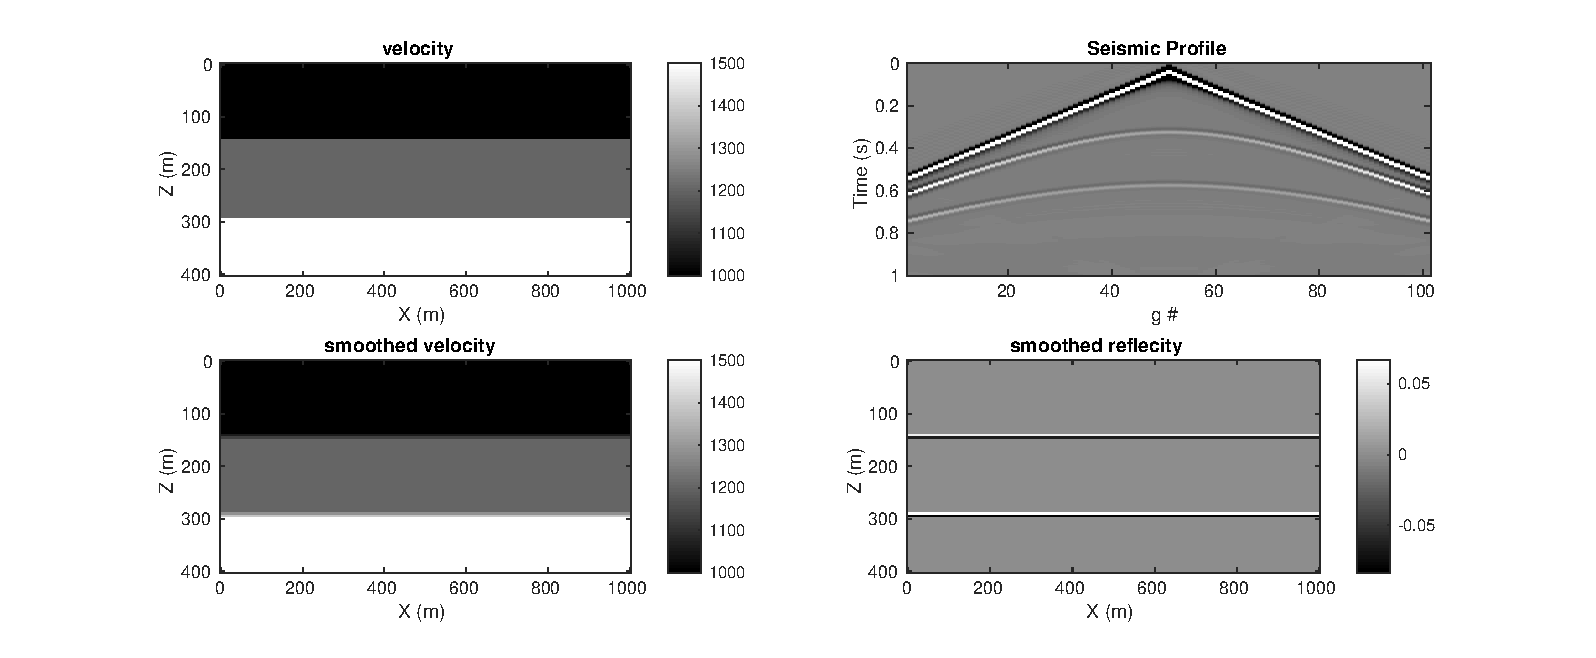
\includegraphics[width=1\linewidth]{./fig/rtm_simuationData.eps}
		\caption{data prepared for RMT}
		\label{rtm_simD}
	\end{figure}

	\subsection{RTM, correlation between D \& U}

	About RTM ,we could derive it from the following relations:\par
	First: we have the relation in frequency domain from  Fréchet derivative\cite{SI}[equation 10.23] and born approximation(consider the source function as $\delta(t)$ and neglect the sum of geophones and sources):
	\begin{align}
		\Delta P(g|s)& =2\omega^2s(x)\Delta s(x)G(g|x)G(x|s)\\
		we\ could\ derive\ :&\notag\\
		\frac{\partial P(g|s)}{\partial s(x)}&=2s(x)\omega^2G(g|x)G(x|s) \label{FE}
	\end{align}

	Before considering the meaning of RTM, we define a loss function of to get the model(use conjugate of P to make sure result is real:
	$$\epsilon=1/2 \int_{\omega}\Delta P(g|s)^* \Delta P(g|s) $$
	get:
	\begin{align}
		\frac{\partial \epsilon}{\partial s(x)}
		&=\int_{\omega}\frac{\partial P(g|s)}{\partial s(x)}^* \Delta P(g|s)\\
		&=2s(x)\int_{\omega}\omega^2G(g|x)^*G(x|s)^* \Delta P(g|s) \\
		&=2s(x)\int_{\omega}G(x|s)^* [G(g|x)^* \omega^2\Delta P(g|s)]
	\end{align}
	we want to get the equation in time domain:
	\begin{align}
		\frac{\partial \epsilon}{\partial s}
		&=-2s(x)\int_{t} D(x,t) \star U(x,t)\\
		D(x,t)=G(x,t|s,0)&,\ U(x,t)=-\mathcal{F}^{-1}[G(g|x)^* \omega^2\Delta P(g|s)] \notag
	\end{align}
	$D(x,t)$ means the forward wavefield from source (when we add the neglected source function to D); and about $U(x,t)$:
	\begin{align}
		U(x,t) 
		& = G(g,-t|x, 0) * \Delta P''(g,t|s,0) \notag\\
		& = G(x,-t|g, 0) * \Delta P''(g,t|s,0) \label{BP-G}\\
		& = G(x,t|g, 0) * d''(g,t)\label{BP-S}\\
		& d''(g,t)= \Delta P''(g,-t|s,0)\notag
	\end{align}

	From \autoref{BP-S}, we can see that if we consider $d''(x,t)$as a source, $U(x,t)$ means a wavefield from geophones with the source $d''(x,t)$, while $d''(x,t)$ is reverse $\Delta P''(t)$ in time. But If we consider from \autoref{BP-G}, $U(x,t)$ is the backpropagated wavefield from geophones. \autoref{BP-S} gives us a method to compute the BP wavefield.\par If we want to iterize the $s(x)$ to make $\epsilon$ smaller, we can use:
	\begin{align}
		s^{i+1}(x) &= s^i(x)-\alpha \frac{\partial \epsilon}{\partial s^i}\\
				   &= s^i(x)+2\alpha s(x)\int_{t} D(x,t) \star U(x,t)
	\end{align}
	$$$$

	Back to RMT, the imagration's definition in RTM is :
		\begin{align}
			m_{mig} &= \frac{s^{1}(x)-s^0(x)}{2\alpha} \notag\\
					&= s^0  	(x)\int_{t} D(x,t) \star U(x,t)dt
		\end{align}
	with all sources and geophones:
		\begin{align}
			m_{mig}(x) &= s(x)\sum_s \sum_g\int_{t} D_s(x,t) \star U_g (x,t)dt \notag\\
					   &= s(x)\sum_s \int_{t} \big[G(x,t|s,0)*W(t|s)\big] \star \sum_g \big[G(x,t|g, 0) * d''(g,t)\big]dt
		\end{align}\par
	
	In applications, we can get $d''(t)$ and the approximated $s(x)$ and $W(t)$. If we want to use RTM to only get the location of reflection:
	\begin{itemize}
		\item \textbf{smooth V} make sure the downgoing wavefield of source have no reflection to geophone
		\item \textbf{mute the diret wave} we only want the reflection part of wavefield, so we can calculate the directive wave$d_d$ and then make $d''=d''-d_d$
		\item \textbf{illumination compensation}\footnote{my question is: do we need to calculate difference A(x) for difference sources?} with the increasing of distance from source, the amplitude will decrease, so the $m_{mig}$ will decrease with depth. So we compensate $m_mig(x)$ with the $A(x)^2$ in wavefield from source, that is:
		$$m_{mig}(x)=\frac{m_{mig}}{A(x)^2}\approx\frac{m_{mig}}{\sum_t D^2(x,t)}$$
		\item \textbf{wavefield reconstruction} when we calculate $d''(g,t)$, we can get $D(x,t)$ and use it to dio corralation with $U(x,t)$. But it means we need store the whole time steps of wavefield, which could be difficult. So some times, we will only store the last two steps in $D(x,t)$ and all boundary condition, to backpropagate.
	\end{itemize}

	\subsection{Figures}
	\begin{figure}[ht]
		\centering
		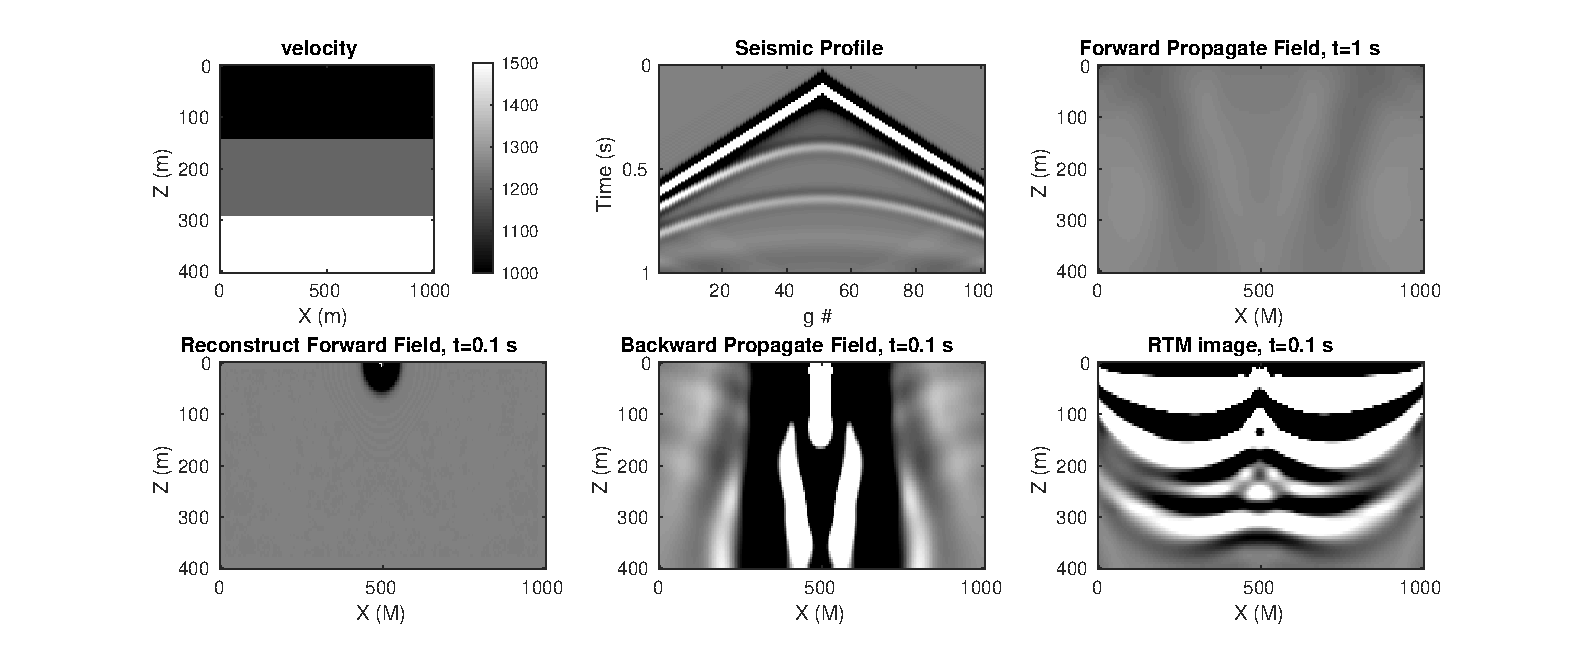
\includegraphics[width=1\linewidth]{./fig/RTM_run_noc.eps}
		\caption{RTM result without direct-wave muting and illumination compensation}
		\label{RTM_noc}
	\end{figure}
	\begin{figure}[ht]
		\centering
		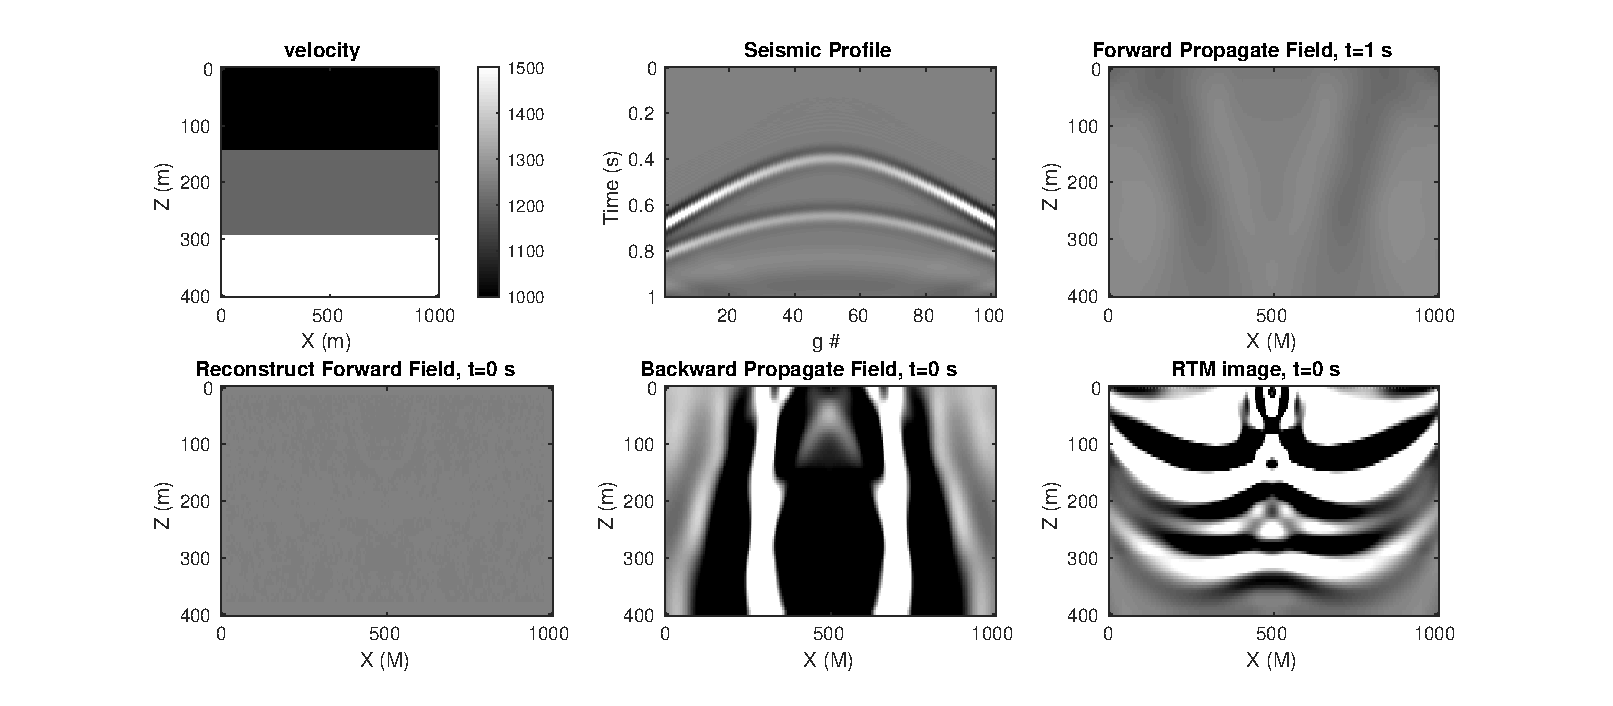
\includegraphics[width=1\linewidth]{./fig/RTM_run_mute.eps}
		\caption{RTM result with direct-wave muting but without illumination compensation}
		\label{RTM_noc_mute}
	\end{figure}

	\begin{figure}[ht]
		\subfigure[IC's impact]
		{
			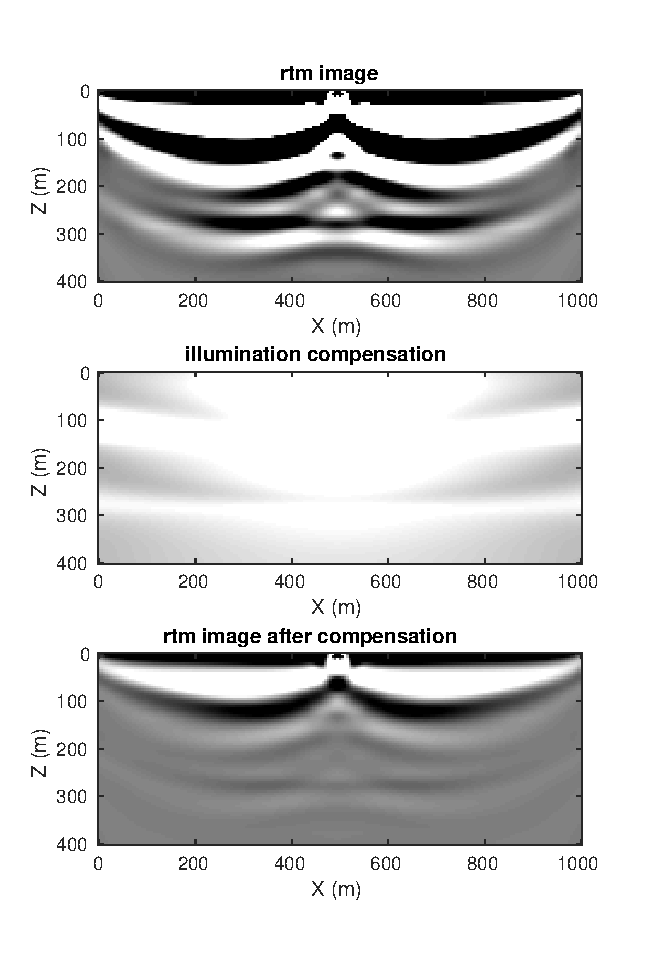
\includegraphics[width=0.5\linewidth]{./fig/RTM_run_c.eps}
			\label{IC_impact}
		}
		\subfigure[IC's impact after muting direct-wave]
		{
			
			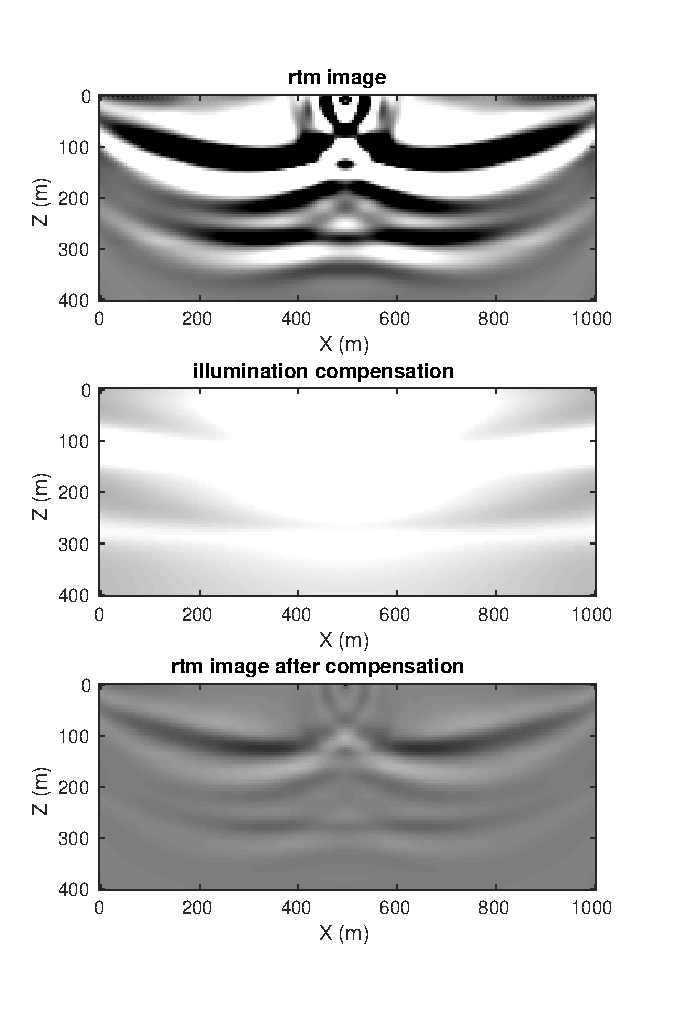
\includegraphics[width=0.5\linewidth]{./fig/RTM_run_mutec.eps}
			\label{IC_impact_mute}
		}

		\centering
		\caption{the impacts of illumination compensation(IC) on the RTM result before \ref{IC_impact} and after \ref{IC_impact_mute} muting direct-wave }
		\label{RTM_c}
	\end{figure}

\clearpage



	

\bibliography{references}
\bibliographystyle{plain}



\end{document}